\PassOptionsToPackage{dvipsnames}{xcolor}


\documentclass{article}


\usepackage[left=3cm,right=3cm,top=2cm,bottom=3cm]{geometry} % page settings
\usepackage{amsmath,amsfonts,amsthm,amssymb} % provides many mathematical environments & tools


\usepackage{tikz}
\usetikzlibrary{shapes,arrows,positioning}
\usetikzlibrary{mindmap,trees, backgrounds}
\usetikzlibrary{decorations.pathreplacing}
\usetikzlibrary{calc}

%\usepackage[dvipsnames]{xcolor}

%\tikzset{block/.style={rectangle, draw, text width=10em, text centered, rounded corners,
 %minimum width=3.5cm}}
 %\tikzset{blockL/.style={rectangle, draw, text width=14em, text centered, rounded corners,
 %minimum width=3.5cm}}
%\tikzset{block_color/.style={rectangle, draw, fill=BurntOrange!65, text width=10em, text centered, rounded corners,
 %minimum width=3.5cm}}
 %\tikzset{line/.style={draw, -latex}}
 
 %\definecolor{green_m}{rgb}{0.0, 0.66, 0.47}
 
 
%\usepackage{adjustbox}

\usepackage{bigints}
\usepackage{hyperref}
%\newcommand{\lver}{\left|}
%\newcommand{\rver}{\right|}
%\newcommand{\bsy}[1]{\boldsymbol{#1}}

\usepackage{hyperref}
\hypersetup{%
  colorlinks=false,% hyperlinks will be black
  linkbordercolor=black,% hyperlink borders will be red
  pdfborderstyle={/S/U/W 1}% border style will be underline of width 1pt
}


% hyperref
\usepackage[]{hyperref}

% color box
%\newcommand{\boxcolor}{orange}
\makeatletter
%\renewcommand{\boxed}[2]{\textcolor{#2}{%
%\tikz[baseline={([yshift=-1ex]current bounding box.center)}] \node [thick, rectangle, minimum width=1ex,rounded corners,draw] {\normalcolor\m@th$\displaystyle#1$};}}



 \makeatother
\begin{document}

\title{Deep Learning Mini-Project 2 Report \\ Implementing from Scratch a Mini Deep-Learning Framework.}
\author{Group 78\footnote{As agreed with Dr. F. Fleuret, L. Pegolotti has collaborated with group 78 for Project 1 and with group 79, with M. Martin, for Project 2. C. Bigoni and N. Ripamonti have worked together on both projects.}  \\ Caterina Bigoni and Nicol\`o Ripamonti}
\date{18 May 2018}
\maketitle
%\tableofcontents
%\newpage



% \small{\textsuperscript{a}EPFL-SB-MATH-MCSS, \textsuperscript{b}EPFL-SB-MATH-DIV}


\section{Introduction}

\section{Code}
The library handles the network structure by means of dictionaries, the ideal type to represent graphs in Python language . The generic dictionary that we have considered can be written as
\begin{align*}
\text{Dictionary} =  \{  & \text{ key}_1  \: : [ \text{ value}_{1,1},  \text{ value}_{1,2}, \dots] ,  \\
&  \text{ key}_2  \: : [ \text{ value}_{2,1},  \text{ value}_{2,2},  \dots] , \} \\
& \dots \\
& \text{ key}_N  \: : [ \text{ value}_{N,1},  \text{ value}_{N,2},  \dots] , \},
\end{align*}
where for each key we may have an arbitrary (and possibly different) number of values. We use the list constructor $[ \dots ]$ to gather all the values related to a certain key because lists are containers easily iterable and we need this feature as explained later on. \\
The first dictionary that has to be defined by the user, called \verb|operators| in \verb|test.py|, is the one that records the modules used in the network. Let us consider a simple network, as the one represented in Figure \ref{example_graph}.
The related dictionary is
\begin{align*}
\text{operators} =  \{  & 1  \: :  \text{ Linear1 }  , \: 2  \: : \text{ Nonlinear1 }   , \\
&  3  \: :  \text{ Linear2 }   , \: 4  \: : \text{ Nonlinear2 }  , \} \\
&   5  \: :  \text{ Sum }   , 1  \: :  \text{ Linear3 }  \}.\\ 
\end{align*}
The next step is the definition of a \verb|connectivity| dictionary: from this variable, an object of the class \verb|Network|, will generate two additional dictionaries, used to introduce and ordering in the forward pass. Since more than 
 \begin{figure}[h]
 \begin{center}
  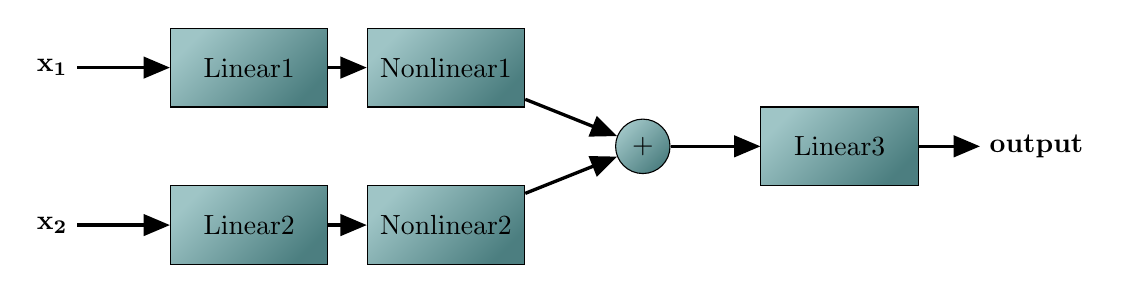
\begin{tikzpicture}
    %%Create a style for the arrows we are using
    \tikzset{normal arrow/.style={draw,-triangle 45,very thick}}
    %%Create the different coordinates to place the nodes
    \coordinate (1) at (0,0);
    \coordinate (2) at (2.5,0);
    \coordinate (3) at (2.5,-2);
    \coordinate (4) at (0,-2);
    \coordinate (5) at (5,-1);
    \coordinate (6) at (7.5,-1);
    \coordinate (x1) at (-2.5,0);
    \coordinate (x2) at (-2.5,-2);
    \coordinate (out) at (10,-1);
    %% Draw nodes
        \node[draw,rectangle,shading=axis,top color=CadetBlue!60, bottom color=CadetBlue!80!black,shading angle=45,minimum width = 2cm, minimum height = 1cm] (n1) at (1) {Linear1};
        \node[draw,rectangle,shading=axis,top color=CadetBlue!60, bottom color=CadetBlue!80!black,shading angle=45,minimum width = 2cm, minimum height = 1cm] (n2) at (2) {Nonlinear1};
        \node[draw,rectangle,shading=axis,top color=CadetBlue!60, bottom color=CadetBlue!80!black,shading angle=45,minimum width = 2cm, minimum height = 1cm] (n3) at (3) {Nonlinear2};
        \node[draw,rectangle,shading=axis,top color=CadetBlue!60, bottom color=CadetBlue!80!black,shading angle=45,minimum width = 2cm, minimum height = 1cm] (n4) at (4) {Linear2};
         \node[draw,circle,shading=axis,top color=CadetBlue!60, bottom color=CadetBlue!80!black,shading angle=45] (n5) at (5) {+}; 
         \node[draw,rectangle,shading=axis,top color=CadetBlue!60, bottom color=CadetBlue!80!black,shading angle=45,minimum width = 2cm, minimum height = 1cm] (n6) at (6) {Linear3};         
        \node (nx1) at (x1) {$\mathbf{x_1}$};
        \node (nx2) at (x2) {$\mathbf{x_2}$};
        \node (xout) at (out) {$\mathbf{output}$};
    %%Drawing the arrows
    \path[normal arrow] (nx1) -- (n1);
    \path[normal arrow] (nx2) -- (n4);
    \path[normal arrow] (n1) -- (n2);
    \path[normal arrow] (n4) -- (n3);
    \path[normal arrow] (n2) -- (n5);
    \path[normal arrow] (n3) -- (n5);
    \path[normal arrow] (n5) -- (n6);
    \path[normal arrow] (n6) -- (xout);
  \end{tikzpicture}
  \caption{Example of network that can be represented using our library.}
  \label{example_graph}
  \end{center}
\end{figure}  

\subsection{General Network}

\subsection{Modules}
With the term \emph{module} we mean each possible element of the network from linear/nonlinear layers to the loss function. Moreover, other operators such as the sum of two different inputs are treated as modules, and hence we obtain an easier representation for more complex networks 3 .
The general structure of a module object is given in \verb|ModuleBase.py| and in each derived object we have to define the following methods:
\begin{itemize}
\item \verb|forward|: Implement the forward pass given the input of the module and store both the input and the output as attributes of the class. 
\item \verb|backward|: Compute the gradient of the loss with respect to the input given the gradient of the loss with respect to the output. If the module contains parameters, it also computes the gradient of the loss with respect of them.
\item \verb|update_param|: Given a learning rate as input, updates the parameters of the module using a gradient descent based approach.
\end{itemize}
\subsubsection{Linear Layer}




\section{Numerical Experiments}

 \section{Conclusion}\label{sec_conclusion}
 
 
 % References
\bibliographystyle{abbrv}
\bibliography{mybib_dl} 
  
  
  
\end{document}